\begin{frame}[t]{Estado del Arte}
	\begin{table} [h!]
		\centering
		\resizebox{\textwidth}{!}{%
			\begin{tabular}{C{0.6\textwidth} C{0.4\textwidth}}
				\normalsize{\textbf{Algoritmos dominio público}} & \normalsize{\textbf{Algoritmos privativos}} \\ \bottomrule
			\end{tabular}
		}
	\end{table}
	\begin{columns}
		\begin{column}{0.6\textwidth}
			\centering
			\vspace*{-10pt}
			\begin{figure}[ht!]
				\centering
				\begin{subfigure}[t]{0.45\textwidth}
					\centering
					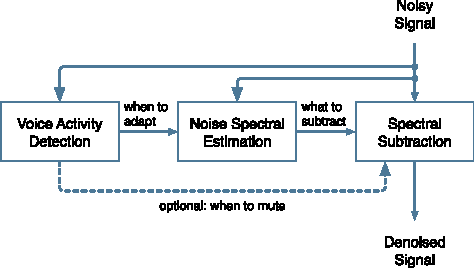
\includegraphics[width=0.9\textwidth]{../figures/rnn_structure.pdf}
					\caption{Estructura del algoritmo presentado por Jean-Marc Valin}
					\label{fig: rnn_structure}
				\end{subfigure}%
				\hspace*{10pt}
				\begin{subfigure}[t]{0.45\textwidth}
					\centering
					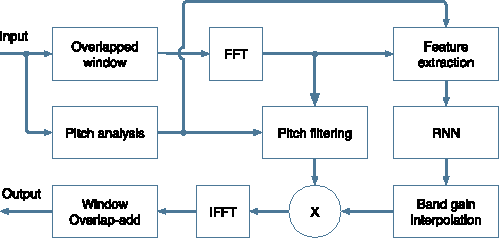
\includegraphics[width=0.9\textwidth]{../figures/rnn_block_diagram.pdf}
					\caption{Diagrama de bloques del eliminación de ruido en el dominio de la frecuencia}
					\label{fig: rnn_block_diagram}
				\end{subfigure}
				\begin{subfigure}[b]{0.65\textwidth}
					\centering
					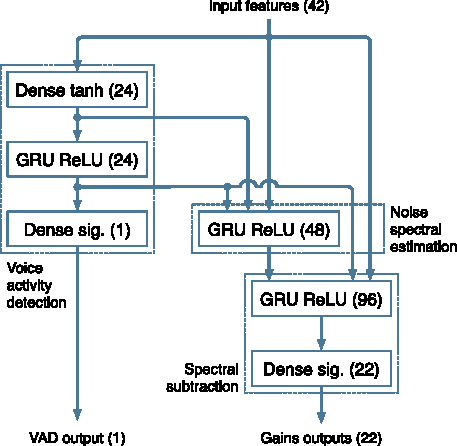
\includegraphics[width=0.9\textwidth]{../figures/rnn_nn.pdf}
					\caption{Red neuronal de RNNoise}
					\label{fig: rnn_nn}
				\end{subfigure}
			\end{figure}
		\end{column}
		\vrule{}
		\begin{column}[t]{0.4\textwidth}
			\vspace*{-100pt}
			\begin{itemize}
				\item \textbf{RTX Voice}
				\begin{itemize}
					\scriptsize
					\item Producto de NVIDIA
					\item \checkTikz{0.2}Gratuito
					\item \redcrossTikz{0.2}Plugins para algunas aplicaciones de chat por voz
					\item \redcrossTikz{0.2}Necesita una gráfica NVIDIA RTX
				\end{itemize}
				\item \textbf{Krisp}
				\begin{itemize}
					\scriptsize
					\item Producto de Krisp
					\item \redcrossTikz{0.2}De pago (gratuito hasta 120$\frac{min}{semana}$)
					\item \checkTikz{0.2}Funciona con el dispositivo de audio del sistema operativo, luego funciona con todo
					\item \checkTikz{0.2}No necesita hardware dedicado
				\end{itemize}
			\end{itemize}
		\end{column}
	\end{columns}
\end{frame}